\section{Auto Organização em RSSF}

 Auto organização é um processo pelo qual estrutura e funcionalidade (padrão) em nível global de um sistema emergem unicamente de numerosas interações entre componentes de baixo nível de um sistema sem qualquer controle externo ou centralizado. Os componentes do sistema interagem em um contexto local por meio de comunicação direta ou observações ambientais sem referência a um padrão global \cite{Dressler2008}.
 
 \subsection{Protocolos MAC auto organizáveis}
 
 A utilização de auto organização em redes de sensores sem fio possibilita ganhos em certos atributos dessas redes, como escalabilidade, consumo de energia, tolerância a falhas, etc. Em protocolos de acesso ao meio, auto organização é utilizada em mecanismos como: atribuição de recursos aos nós \cite{Dressler2008}, determinação de ciclos de sono%
 % FOOTNOTE begin 
 \footnote{Com o objetivo de aumentar o tempo de vida útil das RSSF são utilizados ciclos de sono (\textit{sleep-wakeup cycle} ou \textit{duty cycle}) onde cada nó é ligado apenas por um curto período de tempo (\textit{wakeup}) e então desligado novamente (\textit{sleep}). A utilização desses ciclos pode aumentar a vida útil das RSSF, devido à redução do consumo de energia durante o período de sono \textit{sleep}, de poucos dias para vários meses ou mesmo anos dependendo da razão entre o tempo em que o nó permanece ligado e o tempo em que permanece desligado.}
 % FOOTNOTE end
 \cite{Halkes:2005}, roteamento de pacotes, etc. Existem muitos exemplos de protocolos de controle de acesso ao meio que utilizam esse tipo de organização para diversos fins, abaixo estão apresentados alguns desses protocolos e o modo como a auto organização é empregada neles.
 
 \subsubsection{WiseMAC}
 
 WiseMAC é baseado em técnicas de amostragem de preâmbulo%
  % PREÂMBULO 
 \footnote{Preâmbulo é um fluxo de dados utilizado para comunicar a intenção de transmitir. Tem duração variável de acordo com o período de sono, pois é preciso garantir que o destinatário receba esse preâmbulo e identifique-se como receptor dos pacotes de dados que serão enviados em seguida.} 
 %
. Através da verificação periódica do meio em busca de atividades de comunicação \cite{El-Hoiydi2004}. Tal verificação consiste em uma varredura de curta duração do canal de rádio. Cada nó verifica o meio com um mesmo período constante \textit{Tw} (Figura ~\ref{fig:wisemac}). Se o meio está ocupado, o nó sensor continua a ouvi-lo até receber um quadro de dados ou até o meio ficar desocupado novamente. Antes de cada quadro de dados ser enviado, o ponto de acesso (\textit{access point}) envia um preâmbulo com a mesma duração do período de verificação para garantir que o receptor esteja acordado no momento em que o quadro de dados for enviado. Essa técnica promove um baixo consumo de energia quando o canal está desocupado, porém tem como desvantagem o fato de que os preâmbulos utilizados podem causar limitações à velocidade de transmissão entre pontos distantes e maior consumo de energia devido a sobrecarga nos receptores e ao fato de todos os nós permanecerem ouvindo essa transmissão (\textit{overhearing}). Um ganho considerável é conseguido ao fazer com que os pontos de acesso conheçam os ciclos de verificação dos outros nós pois ele poderá iniciar transmissões somente no momento em que os outros nós estarão ouvindo.
 
\begin{figure}[!htb]
\centering
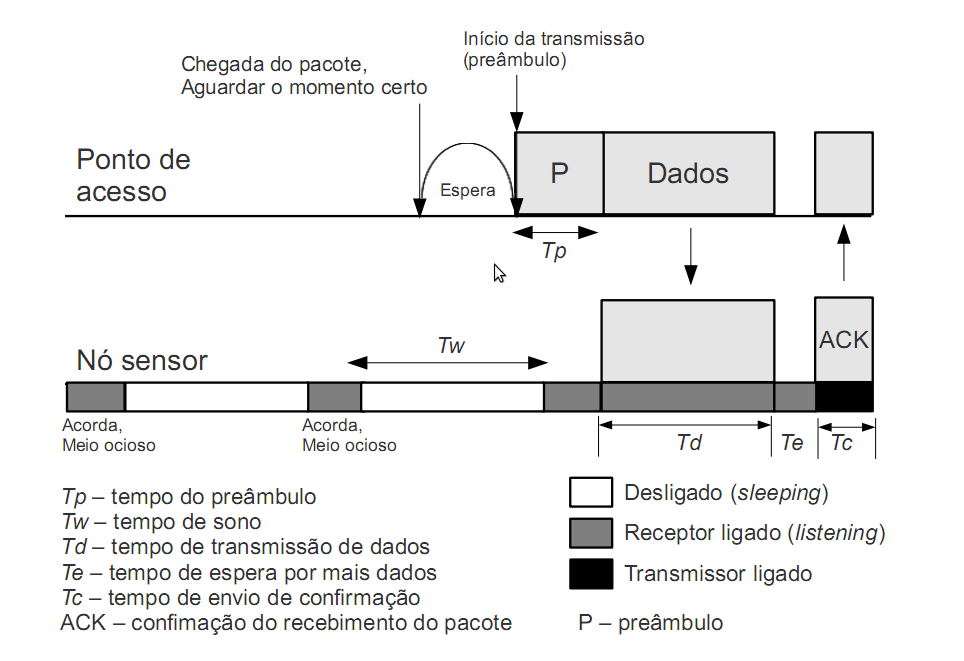
\includegraphics[width=340px,height=220px]{./Pictures/wisemac.png}
% SensorNodesScatteredInASensorField.png: 816x1056 pixel, 96dpi, 21.59x27.94 cm, bb=0 0 612 792
% pdfLaTeX aceita figuras no formato PNG, JPG ou PDF
% figuras vetoriais podem ser exportadas para eps e depois convertidas para pdf usando epstopdf
\caption{Funcionamento do WiseMAC \cite{El-Hoiydi2004}.} %legenda
\label{fig:wisemac} %rotulo para refencia
\end{figure}

 \subsubsection{S-MAC}
 \label{sec:smac}
 
Sensor-MAC ou S-MAC foi desenvolvido para ter primordialmente baixo consumo de energia, além disso conseguiu-se também boa escalabilidade e baixo número de colisões \cite{ye04}. Para conseguir esse resultados foram tratados os seguintes problemas identificados pelo autor como responsáveis pelo consumo excessivo de energia na rede: colisões de pacotes, que causam a retransmissão desses pacotes e consequente consumo extra de energia além de aumentar a latência na rede; \textit{overhearing}, que acontece quando os nós recebem pacotes que não são destinados a eles; excesso (\textit{overhead}) de pacotes de controle; e \textit{idle listening}, quando um nó permanece em modo de recepção aguardando por pacotes que não são enviados.

Para alcançar esses resultados foi adotado um padrão de ciclos de sono com períodos longos de inatividade (período de sono) e períodos de atividade curtos. Auto organização está presente na sincronização dos períodos de atividade/sono dos nós em uma vizinhança, fazendo com que os nós adotem um mesmo cronograma de funcionamento. Isso possibilita que eles possam se comunicar e transmitir informações com eficiência apesar do maior tempo de inatividade. Além disso pode-se reduzir o tamanho dos preâmbulos pois tem-se uma garantia de que os nós aos quais os dados se destinam estarão acordados no mesmo momento (ou em um momento muito próximo) em que aquele que deseja transmitir.

\begin{figure}[!htb]
\centering
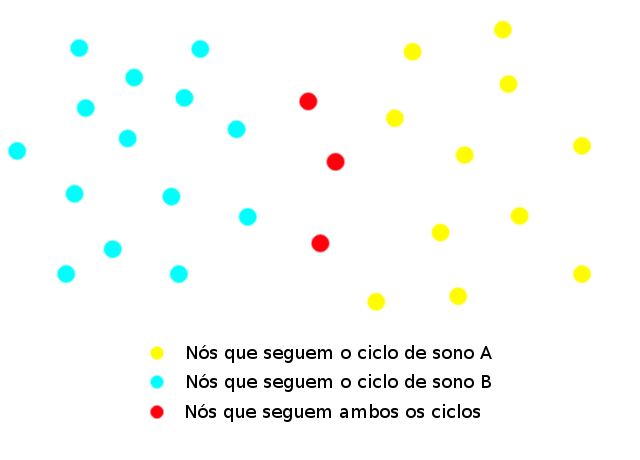
\includegraphics[width=290px,height=180px]{./Pictures/S-MACSynchronization.png}
% SensorNodesScatteredInASensorField.png: 816x1056 pixel, 96dpi, 21.59x27.94 cm, bb=0 0 612 792
% pdfLaTeX aceita figuras no formato PNG, JPG ou PDF
% figuras vetoriais podem ser exportadas para eps e depois convertidas para pdf usando epstopdf
\caption{Exemplo de sincronização de ciclos de atividades com protocolo S-MAC (\emph{clusters} A e B e nós de borda).} %legenda
\label{fig:SmacSynch} %rotulo para refencia
\end{figure}
 
Como desvantagem desse protocolo pode-se destacar que a sincronização dos ciclos de sono se dá entre um certo número de nós de uma região da rede e os nós que ficam no limiar entre duas regiões devem sincronizar-se com ambas as regiões (Figura ~\ref{fig:SmacSynch}). Isso faz com que o consumo de energia desses nós seja maior, reduzindo-se assim o seu tempo de vida útil.
 

%%%%%%%%%%%%%%%%%%%%%%%%Nós sensores são alimentados por baterias, o que faz com que o consumo de energia seja uma restrição muito forte a ser tratada. Crescentes avanços tecnológicos tem tornado o custo de produção dos nós cada vez menor. Em razão disso, tem se tornado cada vez mais vantajoso substituir os nós ao invés de trocar suas baterias, tendo em vista que, na maioria dos casos, eles são inseridos em ambientes que dificultam ou mesmo impossibilitam o procedimento de troca.  
 
 
 
%\subsection{Transceiver operational states} \cite{Karl2005} pdf-p.47



% sensor-MAC (S-MAC), a MAC protocol
% explicitly designed for wireless sensor networks. While re-
% ducing energy consumption is the primary goal in our design,
% S-MAC also achieves good scalability and collision avoidance
% by utilizing a combined scheduling and contention scheme.
% To achieve the primary goal of energy efficiency, we need to
% identify what are the main sources that cause inefficient use of
% energy as well as what tradeoffs we can make to reduce energy
% consumption.
% 
% We have identified the following major sources of energy
% waste. The first one is collision. When a transmitted packet is
% corrupted, it has to be discarded, and follow-on re-transmis-
% sions increase energy consumption. Collision increases latency
% as well. The second source is overhearing, meaning that a
% node picks up packets that are destined to other nodes. The
% third source is control packet overhead. Sending and receiving
% control packets consumes energy too. The last major source of
% inefficiency is idle listening, i.e., listening to receive possible
% traffic that is not sent. This is especially true in many sensor
% network applications. If nothing is sensed, nodes are in idle
% mode for most of the time. 

%\subsection{Ciclos de Sono} 
 
%Com o objetivo de aumentar o tempo de vida útil das RSSF são utilizados ciclos de sono (\textit{sleep-wakeup cycle} ou \textit{duty cycle}) onde cada nó é ligado apenas por um curto período de tempo (\textit{wakeup}) e então desligado novamente (\textit{sleep}). Devido a utilização desse mecanismo, quando um nó precisa transmitir uma mensagem, ele deve permanecer ligado aguardando que seu destinatário também seja ligado e possa receber essa menságem. A utilização desse ciclos pode aumentar a vida útil das RSSF de poucos dias para vários meses ou mesmo anos dependendo da razão entre o tempo em que o nó permanece ligado e o tempo em que permanece desligado. Segundo \cite{1182838}, os parâmetros chave para caracterizar os ciclos de sono incluem tempo desligado (emph{sleep time}), tempo ligado (\textit{wakeup time}), e a energia consumida durante cada um dos estados (ligado/desligado). 
 
%Além da implementação de ciclos de sono também é possível utilizar ouros mecanismos para, em conjunto com ela, permitir um menor consumo de energia através da eliminação ou redução da ocorrência de outros problemas que podem ocasionar o consumo desnecessário de energia, como \textit{overhearing, protocol overhead, collision, idle lisetening, } etc. 
 
%Esse tipo de controle é realizado por protocolos MAC (Medium Access Control - Controle de Acesso ao Meio). Segundo Karl e Willing os protocolos MAC determinam para um nó os pontos no tempo quando ele pode acessar o meio para tentar transmitir dados, controles ou pacotes de gerenciamento para outro nó (unicast) ou para um grupo de nós (multicast, broadcast). 